\documentclass{standalone}
\usepackage{tikz}

\definecolor{purple}{rgb}{0.322, 0.231, 0.412}
\definecolor{red}{rgb}{0.753, 0.2, 0.09}
\definecolor{yellow}{rgb}{0.831, 0.804, 0.349}

\begin{document}
    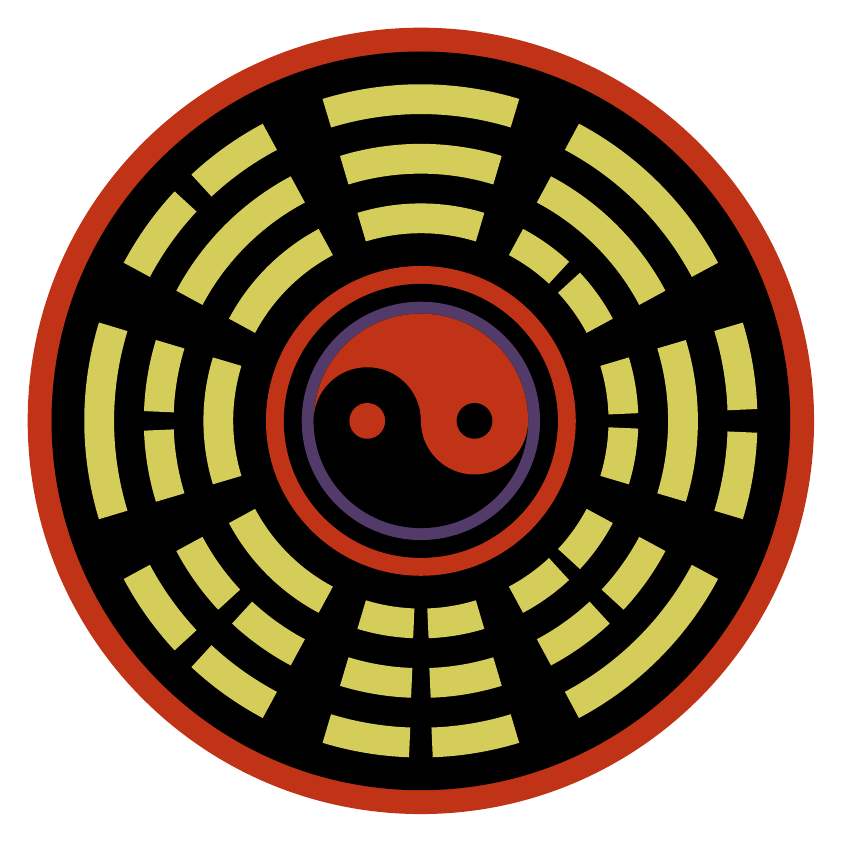
\begin{tikzpicture}
        \draw[draw=none,fill=red] (0,0) circle (33ex);
        \draw[draw=none,fill=black] (0,0) circle (31ex);
        \draw[draw=none,fill=red] (0,0) circle (13ex);
        \draw[draw=none,fill=black] (0,0) circle (11.5ex);
        \draw[draw=none,fill=purple] (0,0) circle (10ex);
        \draw[draw=none,fill=black] (0,0) circle (9ex);
        \draw[draw=none,fill=red] (9ex,0) arc (0:180:9ex);
        \draw[draw=none,fill=black] (-4.5ex,0) circle (4.5ex);
        \draw[draw=none,fill=red] (4.5ex,0) circle (4.5ex);
        \draw[draw=none,fill=red] (-4.5ex,0) circle (1.5ex);
        \draw[draw=none,fill=black] (4.5ex,0) circle (1.5ex);
        
        % full arcs
        \foreach \start/\distance in {73/17ex,118/17ex,163/17ex,208/17ex,73/22ex,118/22ex,-17/22ex,28/22ex,73/27ex,163/27ex,298/27ex,28/27ex}{
            \pgfmathsetmacro{\end}{\start+34}
            \draw[draw=yellow,line width=2.5ex] (\start:\distance) arc (\start:\end:\distance);
        }
        
        % partial arcs
        \foreach \start/\distance in {118/27ex,163/22ex,208/22ex,208/27ex,253/17ex,253/22ex,253/27ex,298/17ex,298/22ex,-17/17ex,-17/27ex,28/17ex}{
            \pgfmathsetmacro{\first}{\start+15}
            \pgfmathsetmacro{\second}{\start+19}
            \pgfmathsetmacro{\end}{\start+34}
            \draw[draw=yellow,line width=2.5ex] (\start:\distance) arc (\start:\first:\distance);
            \draw[draw=yellow,line width=2.5ex] (\second:\distance) arc (\second:\end:\distance);
        }
    \end{tikzpicture}
\end{document}